\chapter{Simulation tools and Introduction to Baadal Architecture}

Getting started with theory of Software defined networking, we tested our grasp on literature by performing simulations with basic topologies and scripts. 

For basic experimentation, we started with the mininet for creating customised topologies using python scripts. Later on we created the baadal architecture using physical host (baadal sandbox).
We will also discuss the baadal networking architecture as a prerequisite to move forward with the installation of baadal sandbox and further development.

\section{Mininet}

Mininet is a network emulator. It creates a network of virtual hosts, switches, controllers, and links. It runs standard Linux network software and supports OpenFlow for flexible custom routing and software defined networking. Some of the features of mininet are: 
\begin{itemize}
    \item A simple and inexpensive \textbf{network testbed} provision for developing OpenFlow applications
    \item Enables complex topology testing, without the need to wire up a physical network
    \item Enables multiple concurrent developers to work independently on the same topology
    \item Provides an extensible Python API for network creation and experimentation
\end{itemize}

\section{Previous work done using mininet: Mini data center simulations}

\begin{figure}[h]
\begin{center}	
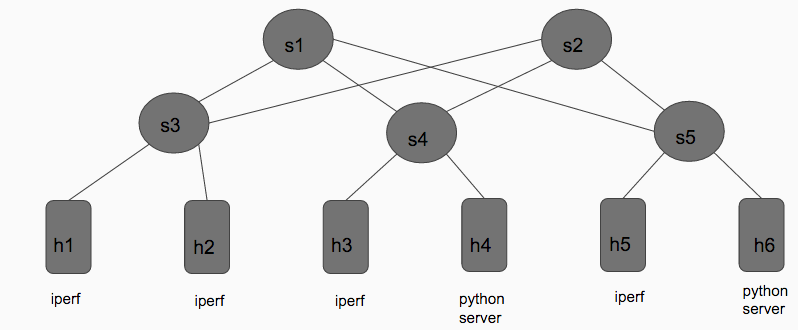
\includegraphics[scale=0.4]{minidc} 
\caption{Data center simulation in mininet}
\label{fig:minidc}
\end{center}
\end{figure}
%\lipsum[2]


\subsection{Mini data center in mininet}
Using the python API of mininet a simulation of a mini data center was done. The topology used is shown in figure \ref{fig:minidc}. It is a classic fat tree topology which is used in many data centers in which the links become thicker as we go from bottom to up. $h_1$ to $h_6$ are hosts which are running different applications . $s_1$ to $s_5$ are the switches present out of which $s_1$ and $s_2$ act as core switches and $s_3$ to $s_5$ act as edge switches. A core switch is a backbone device, a switch that is central to a network’s successful operation. We use it to connect to servers, the Internet service provider (ISP) via a router, and to aggregate all switches that a company uses to connect crucial pieces of equipment that a company can’t afford to lose to downtime. As a result, a core switch should always be a fast, full-featured managed switch. Edge switches, on the other hand, connect client devices, such as laptops, desktops, security cameras, and wireless access points, to the network.

All the hosts except $h_4$ and $h_6$ are running iperf which is a tool to measure bandwidth and quality of network links. $h_4$ and $h_6$ are running a python server and client respectively. Using the controller different statistics were obtained such as the number of bytes transmitted and received by different hosts. In figure \ref{fig:pie} the bandwidth share between different hosts is plotted and in figure \ref{fig:stats} the variation of number of bytes exchanged by the hosts is plotted with respect to time.

\begin{figure}[h]
\begin{center}	

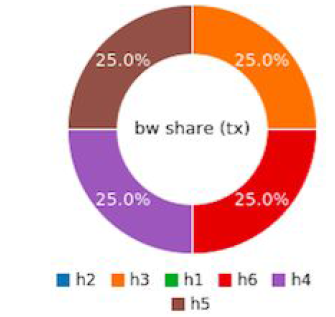
\includegraphics[scale=0.4]{pie} 
\caption{Bandwidth share between different hosts}
\label{fig:pie}
\end{center}
\end{figure}

\begin{figure}[h]
\begin{center}	
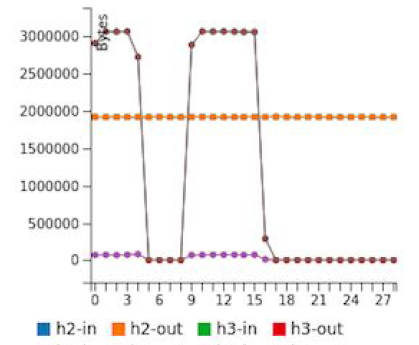
\includegraphics[scale=0.4]{stats} 
\caption{Number of bytes transmitted and received by different hosts}
\label{fig:stats}
\end{center}
\end{figure}

\pagebreak

\begin{figure}[h]
\begin{center}	
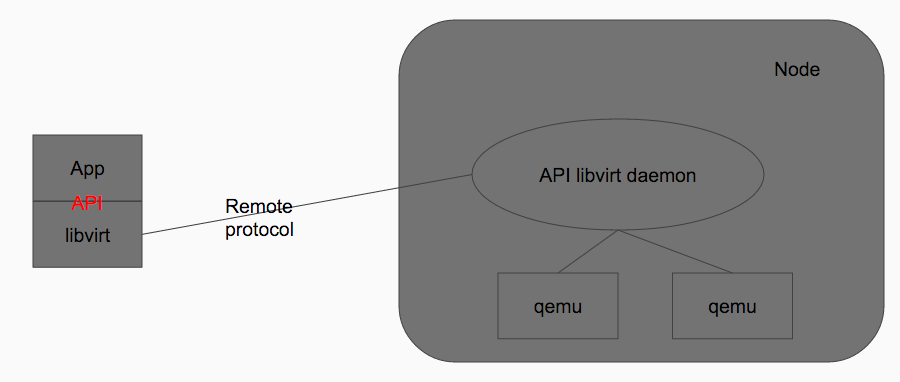
\includegraphics[scale=0.4]{libvirt_arch_1} 
\caption{Libvirt architecture}
\label{fig:libvirt_arch_1}
\end{center}
\end{figure}

\begin{figure}[h]
\begin{center}	
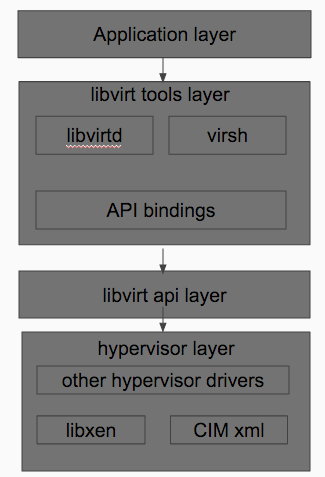
\includegraphics[scale=0.4]{libvirt_arch_2} 
\caption{Libvirt stack}
\label{fig:libvirt_arch_2}
\end{center}
\end{figure}



\subsection{Libvirt}
The libvirt toolkit provides a higher-level VM management interface for
tools and applications, that is:
\begin{itemize}
    \item A set of command line utilities for interacting with the virtualization capabilities of the OS
    \item A consistent set of APIs in C with the aim to provide support across different virtualization tools
\end{itemize}

The goals of libvirt are as follows:
\begin{itemize}
    \item To provide all the operations needed to manage guests or
    domains running on a single physical node
    \item To supply a stable interface that isolates upper-level software
    from changes in the underlying virtualization layer
\end{itemize}
%\lipsum[3]

\subsubsection{Libvirt architecture}
The basic architecture of libvirt is shown in figure \ref{fig:libvirt_arch_1} which shows that the API libvirt daemon runs on a node (a node is a physical machine). It controls the qemu hypervisor on which guests are run. It also has the provision of connecting to the domains over remote protocol call which is a secure link. 

Figure \ref{fig:libvirt_arch_2} shows the libvirt stack:
\begin{itemize}
    \item libvirt: It is the core API layer
    \item virsh: It is a command line program which provides a shell environment and a management user interface using which we can create, pause, list, migrate and shutdown the domains.
    \item libvirtd: It is a daemon (a process which runs in the banckground) for managing guest instances and libvirt virtual networks.
\end{itemize}

\subsubsection{Libvirt connection}
Libvirt makes use of URI to specify which driver a connection refers to driver[+transport]://[username@][hostname][:port]/[path][?extraparameters]. The parameters are defined as follows:
\begin{itemize}
    \item driver : the virtualization technology to interact with
    \item username : the credentials to use for connecting to the driver.
    \item hostname : the (possible remote) host where the virtualization
technology resides
    \item port : the port where the virtualization technology listens for
connections
    \item path : a driver dependent path (e.g. the path to a Unix domain
socket)
    \item extraparameters : additional optional parameters
    \item transport : the transport layer to use for connecting to the driver
\end{itemize}


\subsection{Hands on with libvirt}
Libvirt was installed in the same vagrant box that was used to do the above experiment related to network statistics. Along with that python-libvirt (the python APi for libvirt), qemu, and virt-manager were also installed. virt-manager is a GUI based domain manager. Then a very basic linux distribution - tiny core linux was installed. Tiny core linux is a bare minimum linux distribution. Figure \ref{fig:virt-manager} shown the installation of tiny core linux using the virt-manager gui.
\pagebreak
\begin{figure}[h]
\begin{center}	
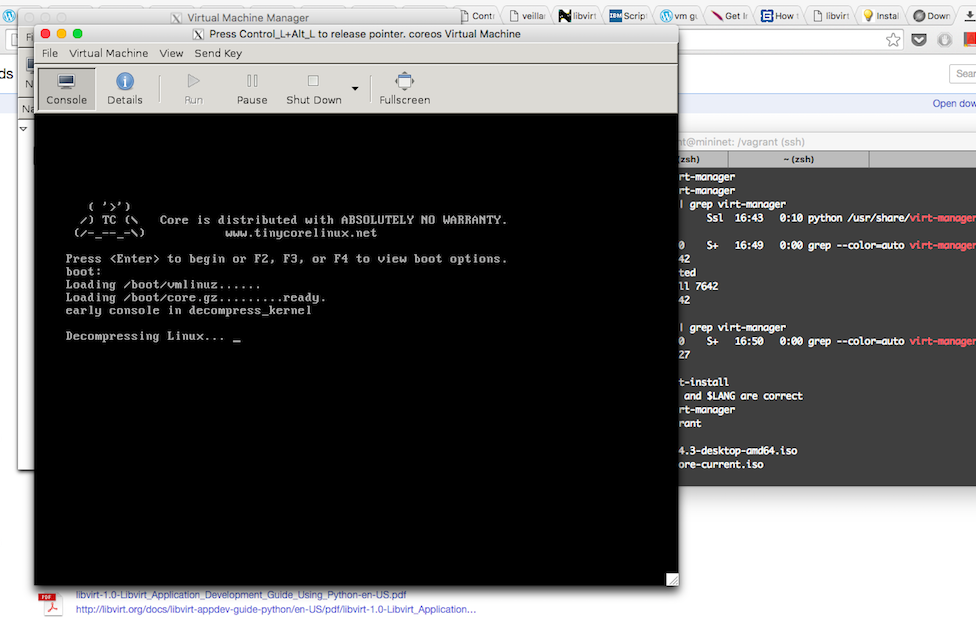
\includegraphics[scale=0.4]{virt-manager} 
\caption{Installation of tiny core linux using virt-manager}
\label{fig:virt-manager}
\end{center}
\end{figure}

\newpage
\subsubsection{CPU statistics}
To get the CPU statistics of the domains using libvirt's python API the function getCPUStats was used. It gives out the time that the domain has consumed out of the CPUs time. This time is in nanoseconds. To convert it into a percentage utilization of CPU we sample the output of getCPUStats every $t$ seconds. Let $cputTimeDiff$ be the change in CPU time over this time $t$ i.e., $cpuTimeDiff = cpuTime_{now} - cpuTime_{now-t}$

Then percentage utilization is calculated as follows \linebreak
$\%CPU utilization = 100 * cpuTimeDiff / (t * number of cores * 10^9)$

\subsubsection{Memory statistics}
To get the memory statistics of the domain using libvirt's python API the function memoryStats can be used. It gives the actual memory that is allotted to the domain, the swap memory and the resident set size is given as the output. Resident set size is the portion of memory occupied by that domain in the main memory (RAM).The rest of the memory may be in swap space or file system. 

\section{Overview of Baadal Networking Architecture}
In this section we will present the overview of the baadal networking architecture. The components comprising the architecture are mentioned below:-

\begin{itemize}
    \item \textbf{NAT} Network Address translator is the component which act as firewall for the baadal network. All the traffic of the baadal network pass through it. Internal baadal nodes communicate to the internet via this interface only. It is implemented on an OpenVswitch which is hosted in a physical machine with Ubuntu as its OS.
    \item \textbf{Hardware Switch} It is a physical switch which is connected to all the other networking components including the physical hosts, Baadal Controller, Filer and NAT.
    \begin{figure}[h]
\caption{Overview of Baadal Architecture}
\centering
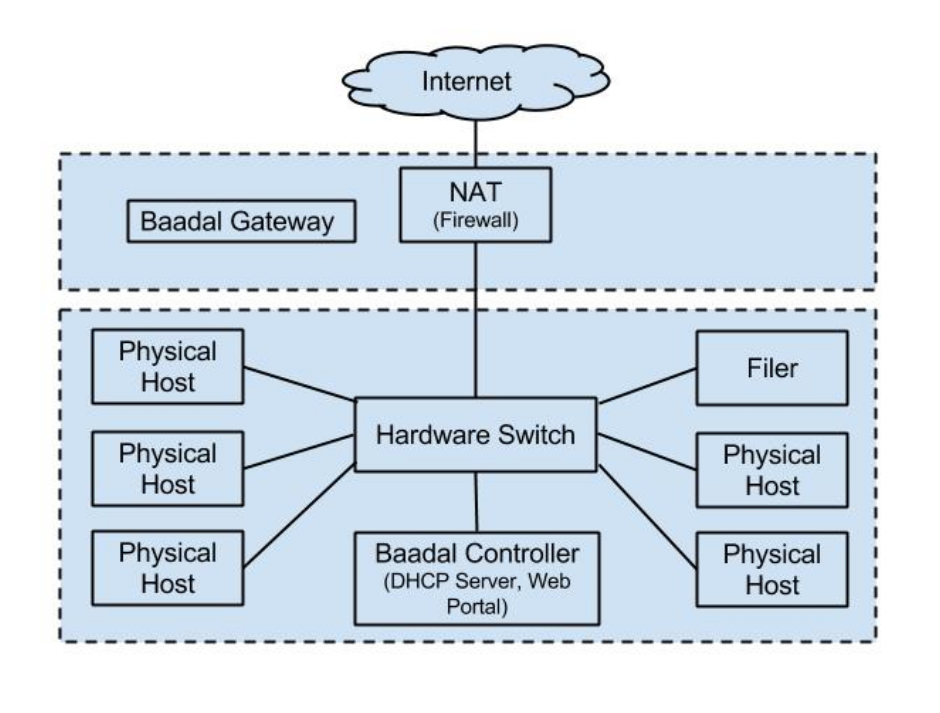
\includegraphics[width=0.9\textwidth]{Baadal_architecture}
\end{figure}
    \item \textbf{Baadal Controller} This component is responsible for providing web portal where a user can request a VM, a facutly supervisor approves it and an administrator can commission it. The main function of it is to be central controlling element alongwith hosting components like DHCP server, TFTP server, scheduler etc.
    
    \item \textbf{Filer} For all the physical hosts Filer is the network file manager. On request of virtual machines, controller hosts the virtual hard disk. But additional hard disk is allocated in the filer machine.
    
    \item \textbf{Physical host} These are responsible for hosting all the VMs created by the user. KVM is the hypervisor layer in the physical host.
    
\begin{figure}[h]
\caption{Physical host architecture}
\centering
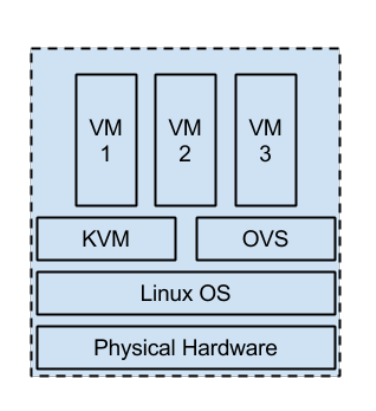
\includegraphics[width=0.5\textwidth]{PhysicalHost_architecture}
\end{figure}
\end{itemize}

%\section{Implementation of Virtual Network using OpenDaylight}